\documentclass[12pt,a4paper]{article}

% ─── Page Layout ───────────────────────────────────────────────────────────────
\usepackage[a4paper, margin=0.8in, headheight=14pt]{geometry}

% ─── Fonts (XeLaTeX) ───────────────────────────────────────────────────────────
\usepackage{fontspec}
\usepackage{unicode-math}
\setmainfont{TeX Gyre Pagella}
\setmonofont[Scale=0.88]{TeX Gyre Cursor}
\setmathfont{Latin Modern Math}

% ─── Packages ──────────────────────────────────────────────────────────────────
\usepackage{xcolor}
\usepackage{colortbl}
\usepackage{titlesec}
\usepackage{enumitem}
\usepackage{tabularx}
\usepackage{longtable}
\usepackage{booktabs}
\usepackage{array}
\usepackage{amsmath}
\usepackage{tikz}
\usetikzlibrary{shapes.geometric, arrows.meta, positioning, calc, fit, decorations.pathreplacing, patterns}
\usepackage{tcolorbox}
\tcbuselibrary{skins, breakable}
\usepackage{hyperref}
\usepackage{fancyhdr}
\usepackage{graphicx}
\usepackage{microtype}
\hyphenpenalty=10000
\exhyphenpenalty=10000
\sloppy
\usepackage{caption}
\usepackage{setspace}
\usepackage{multirow}
\usepackage{tocloft}

% ─── Q&A helper ────────────────────────────────────────────────────────────────
\newcommand{\Q}[1]{\textbf{#1}\par\noindent\ignorespaces}

% ─── Colour Palette ────────────────────────────────────────────────────────────
\definecolor{myred}{RGB}{196,30,58}
\definecolor{mydark}{RGB}{30,30,50}
\definecolor{mygreen}{RGB}{14,120,80}
\definecolor{myteal}{RGB}{0,130,140}
\definecolor{myamber}{RGB}{180,100,0}
\definecolor{mypurple}{RGB}{100,30,160}
\definecolor{mygray}{RGB}{246,247,249}
\definecolor{mgframe}{RGB}{180,185,200}
\definecolor{watermark}{RGB}{145,150,170}
\definecolor{hdrred}{RGB}{250,232,235}
\definecolor{hdrgreen}{RGB}{220,244,233}
\definecolor{hdrteal}{RGB}{220,242,244}
\definecolor{hdramber}{RGB}{253,242,215}
\definecolor{hdrpurple}{RGB}{238,228,255}
\definecolor{hdrgray}{RGB}{238,240,245}

% ─── Section Formatting ────────────────────────────────────────────────────────
\titleformat{\section}
  {\large\bfseries\color{myred}}{\thesection.}{0.5em}{}
  [\vspace{1pt}{\color{myred}\rule{\linewidth}{0.8pt}}]
\titleformat{\subsection}
  {\normalsize\bfseries\color{myteal}}{\thesubsection}{0.5em}{}
\titlespacing*{\section}{0pt}{18pt}{7pt}
\titlespacing*{\subsection}{0pt}{11pt}{4pt}

% ─── Paragraph ─────────────────────────────────────────────────────────────────
\setlength{\parindent}{0pt}
\setlength{\parskip}{4pt}

% ─── TOC Styling ───────────────────────────────────────────────────────────────
\renewcommand{\cfttoctitlefont}{\large\bfseries\color{myred}}
\renewcommand{\cftaftertoctitle}{\par\noindent{\color{myred}\rule{\linewidth}{0.8pt}}}
\setlength{\cftbeforetoctitleskip}{0pt}
\setlength{\cftaftertoctitleskip}{6pt}
\renewcommand{\cftsecfont}{\normalsize\bfseries\color{mydark}}
\renewcommand{\cftsecpagefont}{\normalsize\bfseries\color{mydark}}
\renewcommand{\cftsecleader}{\cftdotfill{\cftdotsep}}
\setlength{\cftbeforesecskip}{7pt}
\renewcommand{\cftsubsecfont}{\small\color{mydark}}
\renewcommand{\cftsubsecpagefont}{\small\color{mydark}}
\setlength{\cftbeforesubsecskip}{3pt}
\setlength{\cftsubsecindent}{1.4em}

% ─── Table helpers ─────────────────────────────────────────────────────────────
\renewcommand{\arraystretch}{1.45}
\setlength{\tabcolsep}{6pt}
\arrayrulecolor{mydark}
\newcolumntype{B}[1]{>{\small\bfseries\raggedright\arraybackslash}m{#1}}
\newcolumntype{Y}{>{\small\raggedright\arraybackslash}X}
\renewcommand{\tabularxcolumn}[1]{m{#1}}

% ─── Header / Footer ───────────────────────────────────────────────────────────
\pagestyle{fancy}
\fancyhf{}
\fancyhead[L]{\small\color{myred}\textbf{BS-B401}\;\color{mydark}--- Biology for Engineers}
\fancyhead[R]{\small\color{myteal}\textbf{Module 7 Notes}}
\fancyfoot[C]{\small\color{mydark}\thepage}
\fancyfoot[R]{\small\color{watermark}\textit{\copyright\ Biraj Sarkar (CGEC)}}
\renewcommand{\headrulewidth}{0.5pt}
\renewcommand{\footrulewidth}{0.3pt}

% ─── Hyperref ──────────────────────────────────────────────────────────────────
\hypersetup{
  colorlinks=true, linkcolor=myteal, urlcolor=myteal,
  pdfauthor={Biraj Sarkar (CGEC)},
  pdftitle={BS-B401 --- Module 7 Notes: Macromolecular Analysis}
}

% ─── tcolorbox styles ──────────────────────────────────────────────────────────
\tcbset{
  tikzbox/.style={
    colback=mygray, colframe=mgframe, boxrule=0.6pt, arc=4pt,
    left=8pt, right=8pt, top=6pt, bottom=6pt,
    colbacktitle=mgframe, coltitle=mydark, fonttitle=\small\bfseries
  },
  defbox/.style={
    colback=hdrgreen, colframe=mygreen, boxrule=0.8pt, arc=4pt,
    left=9pt, right=9pt, top=6pt, bottom=6pt,
    colbacktitle=mygreen, coltitle=white, fonttitle=\small\bfseries
  },
  formulabox/.style={
    colback=hdrteal, colframe=myteal, boxrule=0.8pt, arc=4pt,
    left=9pt, right=9pt, top=7pt, bottom=7pt,
    colbacktitle=myteal, coltitle=white, fonttitle=\small\bfseries
  },
  examplebox/.style={
    colback=hdramber, colframe=myamber, boxrule=0.8pt, arc=4pt,
    left=9pt, right=9pt, top=6pt, bottom=6pt,
    colbacktitle=myamber, coltitle=white, fonttitle=\small\bfseries
  },
  masonbox/.style={
    colback=hdrpurple, colframe=mypurple, boxrule=0.8pt, arc=4pt,
    left=9pt, right=9pt, top=6pt, bottom=6pt,
    colbacktitle=mypurple, coltitle=white, fonttitle=\small\bfseries
  },
  exambox/.style={
    colback=hdrpurple, colframe=mypurple, boxrule=1pt, arc=5pt,
    left=10pt, right=10pt, top=8pt, bottom=8pt,
    colbacktitle=mypurple, coltitle=white, fonttitle=\bfseries,
    breakable, title after break={\textbf{Frequently Asked / Viva Questions (contd.)}}
  }
}
\tcbset{breakable}
\tcbset{after={\par\color{black}}}

% ─── TikZ styles ───────────────────────────────────────────────────────────────
\tikzset{
  block/.style={rectangle, draw=myteal, fill=hdrteal,
    text width=2.4cm, align=center, minimum height=0.95cm,
    font=\small, rounded corners=3pt, line width=0.7pt},
  redblock/.style={rectangle, draw=myred, fill=hdrred,
    text width=2.4cm, align=center, minimum height=0.95cm,
    font=\small, rounded corners=3pt, line width=0.7pt},
  amberblock/.style={rectangle, draw=myamber, fill=hdramber,
    text width=2.4cm, align=center, minimum height=0.95cm,
    font=\small, rounded corners=3pt, line width=0.7pt},
  sumjunc/.style={circle, draw=myamber, fill=hdramber,
    minimum size=0.62cm, font=\small, line width=0.8pt},
  arrow/.style={-Stealth, thick, color=mydark},
  redarrow/.style={-Stealth, thick, color=myred},
  line/.style={thick, color=mydark}
}

\begin{document}

% ─── Title Page ───────────────────────────────────────────────────────────────
\begin{center}
  {\LARGE\bfseries\color{myred} BS-B401 --- Biology for Engineers}\\[5pt]
  {\normalsize\color{mydark} Semester IV \quad$\bullet$\quad 2L:1T:0P \quad$\bullet$\quad 3 Credits}\\[3pt]
  {\normalsize\color{myteal}\textbf{Module 7 Exam Notes: Macromolecular Analysis}}\\[3pt]
  {\small\color{mydark} CGEC \;$|$\; B.Tech ECE (2023--27) \;$|$\; \textit{Biraj Sarkar}}
\end{center}
\vspace{2pt}
\noindent{\color{myred}\rule{\linewidth}{1.5pt}}
\vspace{2pt}

\hypersetup{linkcolor=mydark}
\tableofcontents
\hypersetup{linkcolor=myteal}
\newpage

\section{Macromolecular Analysis}
\subsection{What a reductionistic analysis asks}
\begin{tcolorbox}[defbox, title={Reductionistic analysis}]
Study a complex biological process by isolating its components and asking what each contributes. Combine measurements of the components to explain the behaviour of the whole system. Check whether the isolated behaviour still applies in the cellular context.
\end{tcolorbox}

\begin{enumerate}[leftmargin=*, itemsep=3pt, topsep=4pt]
  \item \textbf{Define the biological task.} For example, ask how a protein recognises oxygen, an ion or a hormone.
  \item \textbf{Identify the component.} Distinguish the polypeptide sequence from its partners, attached small molecules and surrounding membrane or solvent.
  \item \textbf{Compare structures and functions.} Check whether a structural observation predicts a measurable function.
  \item \textbf{Test the explanation.} Compare conditions or naturally occurring variants, then distinguish direct effects on the active site from effects on folding, stability or expression.
\end{enumerate}
\subsection{The four levels of protein structure}
\par\vspace{5pt}
\begingroup
\setlength{\extrarowheight}{1pt}
\noindent\begin{tabularx}{\linewidth}{|B{3.1cm}|Y|Y|}
\hline
\textbf{Level} & \textbf{What is organised} & \textbf{Forces or examples} \\ \hline
Primary & Amino-acid sequence of a polypeptide, written N to C. & Peptide bonds form the backbone. Side-chain order constrains folding. \\ \hline
Secondary & Local backbone patterns such as alpha helices and beta sheets. & Hydrogen bonds between backbone carbonyl and amide groups. Turns connect elements. \\ \hline
Tertiary & Overall three-dimensional arrangement of one polypeptide chain. & Hydrophobic effects, ionic interactions, hydrogen bonds, van der Waals contacts and some disulfide bonds. \\ \hline
Quaternary & Association of several polypeptide chains into one functional assembly. & Interfaces between subunits. Adult haemoglobin has two alpha and two beta chains. \\ \hline
\end{tabularx}\par
\endgroup
\begin{tcolorbox}[tikzbox, title={Read protein structure by scale}]
\centering
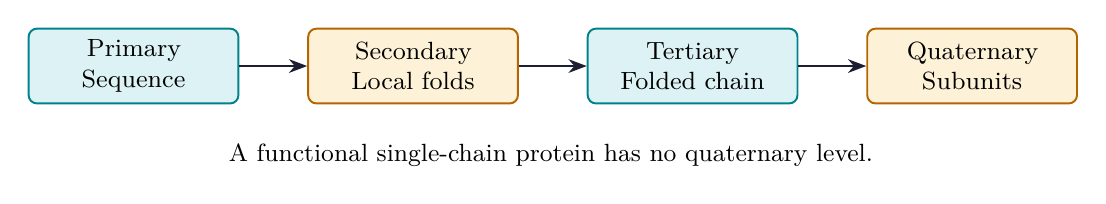
\begin{tikzpicture}[every node/.style={font=\small}]
\node[block,text width=2.43cm] (a) at (0,0) {Primary\\Sequence};
\node[amberblock,text width=2.43cm] (b) at (3.55,0) {Secondary\\Local folds};
\node[block,text width=2.43cm] (c) at (7.1,0) {Tertiary\\Folded chain};
\node[amberblock,text width=2.43cm] (d) at (10.65,0) {Quaternary\\Subunits};
\draw[arrow] (a)--(b);
\draw[arrow] (b)--(c);
\draw[arrow] (c)--(d);
\node at (5.3,-1.13) {A functional single-chain protein has no quaternary level.};
\end{tikzpicture}\par
\end{tcolorbox}

\begin{itemize}[leftmargin=*, itemsep=3pt, topsep=4pt]
  \item \textbf{Alpha helix.} The backbone coils with hydrogen bonds between residues separated by four positions along the chain. Side chains project outward.
  \item \textbf{Beta sheet.} Backbone segments align side by side. Hydrogen bonds connect the strands, which may run parallel or antiparallel.
  \item \textbf{Domains.} A domain is a compact structural unit within a chain. A protein can have several domains with different activities, such as binding and catalysis.
  \item \textbf{Denaturation.} Heat or a chemical change may disrupt native folding and subunit interactions. Ordinary denaturation can abolish activity while leaving most peptide bonds intact.
\end{itemize}
\section{Protein Functions and How to Compare Them}
\subsection{Function depends on structure}
\par\vspace{5pt}
\begingroup
\setlength{\extrarowheight}{1pt}
\noindent\begin{tabularx}{\linewidth}{|B{3.1cm}|Y|Y|}
\hline
\textbf{Role} & \textbf{Structure--function link} & \textbf{Example} \\ \hline
Enzyme & A folded active site brings reactive groups into the right positions. & Carbonic anhydrase accelerates carbon dioxide hydration. \\ \hline
Transporter & A binding site or pore selects a substance. Some transporters use alternating access and energy coupling. & A glucose carrier helps glucose cross a membrane. Haemoglobin transports oxygen in blood. \\ \hline
Receptor & A specific ligand changes the receptor's conformation or interactions and triggers signalling. & The insulin receptor detects insulin and initiates intracellular signalling. \\ \hline
Structural & Fibres and networks resist or distribute forces. & Collagen triple helices contribute to connective-tissue strength. \\ \hline
\end{tabularx}\par
\endgroup
\begin{tcolorbox}[examplebox, title={Separate binding from cooperative behaviour}]
Myoglobin is a single-chain oxygen-binding protein. Haemoglobin contains several subunits. Oxygen binding at one haemoglobin subunit can increase the affinity of the others, giving cooperative binding. This comparison connects a quaternary assembly to a function that cannot be explained by counting identical independent sites alone.
\end{tcolorbox}

\subsection{What common measurements reveal}
\par\vspace{5pt}
\begingroup
\setlength{\extrarowheight}{1pt}
\noindent\begin{tabularx}{\linewidth}{|B{3.6cm}|Y|Y|}
\hline
\textbf{Method} & \textbf{What it can show} & \textbf{Limit} \\ \hline
Gel electrophoresis under denaturing conditions & Approximate chain masses or the presence of several polypeptide species. & Native associations and activity may be lost during analysis. \\ \hline
Size-exclusion chromatography & Relative hydrodynamic size of species in solution. & Shape affects the estimate. Size alone may not establish subunit count. \\ \hline
X-ray crystallography, NMR or cryo-EM & Complementary structural information at different scales and in different conditions. & A structural model must be interpreted with sample conditions and resolution in mind. \\ \hline
Binding or activity assay & Whether ligand binding or catalytic function is measurable. & A low signal may reflect poor folding, low protein amount or a direct functional defect. \\ \hline
\end{tabularx}\par
\endgroup
\begin{tcolorbox}[masonbox, title={Exam response pattern}]
For a structure--function answer, name the structural level, identify the relevant feature, explain the physical consequence, and give a specific biological example.
\end{tcolorbox}

\subsection{Distinguish a channel, a carrier, a pump and a receptor}
\par\vspace{6pt}
\noindent\begin{tabularx}{\linewidth}{|B{3.2cm}|Y|Y|}
\hline
\textbf{Protein role} & \textbf{What changes} & \textbf{What to look for} \\ \hline
Channel & An open pore allows selected ions or molecules through. & Movement through an open channel follows the appropriate electrochemical gradient. \\ \hline
Carrier & A binding site faces one side and then the other. & Binding and conformational change can account for selective, saturable transport. \\ \hline
Pump & Transport is coupled to an energy-yielding process. & An ATP-driven pump can maintain a gradient by moving solutes uphill. \\ \hline
Receptor & A ligand selects or changes a receptor state. & Signal transmission is the defining function. Some receptors also include a channel, so the roles can overlap. \\ \hline
\end{tabularx}\par

\begin{tcolorbox}[examplebox, title={Distinguish binding from signalling}]
Suppose a receptor variant binds the same amount of ligand as the usual receptor but gives a smaller downstream response. Normal binding is evidence that ligand recognition still works under the conditions tested. A changed response suggests a problem with coupling, receptor abundance at the relevant surface, or a downstream partner. Measuring binding alone cannot distinguish these explanations.
\end{tcolorbox}

\subsection{Connect a measurement to the affected structural level}
\begin{enumerate}[leftmargin=*, itemsep=2pt]
  \item \textbf{Check the chain.} If a denaturing measurement shows the expected chain mass, major loss of the polypeptide is less likely. That result alone does not establish correct folding.
  \item \textbf{Check the assembly.} A structural or solution measurement can indicate whether the expected subunits associate. Different assemblies can contain the same chain types.
  \item \textbf{Check function.} Read out binding, catalytic activity or transport, and compare the result with the structure. An unchanged sequence can still yield a different response if the environment or assembly differs.
  \item \textbf{Apply this to haemoglobin.} A single chain can bind oxygen with its haem group. The multi-subunit assembly lets binding at one site influence other sites, which explains why the response depends on more than the number of binding sites.
\end{enumerate}

\newpage
\begin{center}
  {\large\bfseries\color{myred} Quick Revision --- Module 7}\\[3pt]
  {\small\color{mydark} Macromolecular Analysis $|$ BS-B401}
\end{center}
\noindent{\color{myred}\rule{\linewidth}{1.2pt}}\par\vspace{4pt}

\begin{tcolorbox}[formulabox, title={Key Concepts at a Glance}]
\renewcommand{\arraystretch}{1.35}
\noindent\begin{tabularx}{\linewidth}{B{4.5cm}Y}
Primary to quaternary & Sequence, local backbone pattern, one chain's fold, then any subunit assembly. \\[3pt]
Hydrogen bonding & Backbone hydrogen bonds stabilise alpha helices and beta sheets. \\[3pt]
Function & Identify the site, interaction or assembly that enables the task. \\[3pt]
\end{tabularx}\par
\end{tcolorbox}

\begin{tcolorbox}[defbox, title={One-Line Definitions}]
\begin{itemize}[leftmargin=*, itemsep=3pt, topsep=4pt]
  \item \textbf{Domain.} Compact structural unit within a protein chain.
  \item \textbf{Denaturation.} Loss of native structure and often activity.
  \item \textbf{Cooperativity.} Binding at one site influences binding at another.
\end{itemize}
\end{tcolorbox}

\begin{tcolorbox}[exambox, title={Frequently Asked / Viva Questions}]
\begin{enumerate}[topsep=0pt, label=\textbf{Q\arabic*.}, itemsep=5pt, leftmargin=*]
  \item \Q{What is primary structure?}
    The amino-acid order in a polypeptide.
  \item \Q{What stabilises regular secondary structures?}
    Hydrogen bonds between backbone groups.
  \item \Q{How do tertiary and quaternary structure differ?}
    Tertiary structure is one chain's fold. Quaternary structure describes multiple subunits.
  \item \Q{Which protein illustrates an alpha-two beta-two assembly?}
    Adult haemoglobin.
  \item \Q{Does denaturation necessarily break peptide bonds?}
    Most peptide bonds may remain intact while folding is lost.
  \item \Q{What structural feature often determines enzyme specificity?}
    The shape and chemistry of the active site.
  \item \Q{How does a receptor act?}
    Ligand recognition changes its state and initiates signalling.
  \item \Q{Give a structural protein example.}
    Collagen.
  \item \Q{Why compare structure with an activity assay?}
    The structure suggests a mechanism. The assay tests whether it functions.
  \item \Q{What does a reductionistic study still need to consider?}
    Interactions and conditions that matter in the intact system.
\end{enumerate}
\end{tcolorbox}

\begin{tcolorbox}[tikzbox, title={Summary Comparison}]
\par\vspace{5pt}
\begingroup
\setlength{\extrarowheight}{1pt}
\noindent\begin{tabularx}{\linewidth}{|B{3.45cm}|Y|Y|}
\hline
\textbf{Level} & \textbf{Subject} & \textbf{Example} \\ \hline
Secondary & Local backbone geometry & Alpha helix. \\ \hline
Tertiary & One chain's three-dimensional fold & Folded myoglobin. \\ \hline
Quaternary & Multiple chains & Haemoglobin assembly. \\ \hline
\end{tabularx}\par
\endgroup
\end{tcolorbox}

\end{document}
